
\section{Design}

In this section, we discuss the planned design of our system. We start by outlining a very high-level architecture of interconnected components that make up our system in the \textit{System Architecture} subsection. Next, we discuss the external tools that will be used to facilitate the development and execution of each component in the \textit{Technology Used} section. In the \textit{Schema/Data Structures} section, the details on how each component represents information is clarified. Finally, in the \textit{Data Flow} section, we elaborate on the specifics of how the separate components communicate with each other.

\subsection{System Architecture}

The architecture of this project is separated into three interconnected components. One component retrieves and stores information on stock prices from various sources so that it can be easily queried on-demand by other components. Another component implements the opinion aggregation model from a related work. The remaining component is responsible for testing a trading strategy and analyzing the results.

\subsubsection{Pricing Data}

The Pricing Data component contains utilities that can be used to query stock prices from a given data source. All stock prices from each source are preloaded into separate tables in an HBase \cite{hbase} database. For our tests, we download data from our sources on the set of stocks that we are testing on (see Table~\ref{tab:stocks}) for the entire year of 2014. Once we have downloaded the data, we can populate a table on the cluster provided to us by Virginia Tech with the price information so that it is in a standardized format. The main purpose of this component is to provide facilities for other components to access stock price information.

\subsubsection{Opinion Aggregation}

The Opinion Aggregation component is an implementation of the model described by Qianzhou Du, Hong Hong, G. Alan Wang, Pingyuan Wang, and Weiguo Fan in \textit{CrowdIQ: A New Opinion Aggregation Model} \cite{crowdiq}. It provides utilities that aggregate an opinion towards a stock symbol based on the microblog posts in a given time interval as well as the historical performance and consistency of each microblog author. This component is also responsible for storing and querying microblog posts from our database and provides utilities for other components to do so as well. Finally, it also provides an implementation of a sentiment analysis utility that categorizes microblog posts as ``bullish'' or ``bearish''.

\subsubsection{Trading Simulation}

The Trading Simulation component brings the other two components together to provide a full simulation of a trading environment. This involves implementing a virtual stock portfolio and the ability to execute transactions to buy and sell stocks. Additionally, it involves the ability to define a strategy that responds to specific events (for example, a microblog post, a stock price change, and/or market open or close events). This component provides utilities that allow you to define a strategy like an event listener which manipulates a virtual portfolio. Within this component, we will also implement the strategies that we are evaluating.

\subsection{Technology Used}

In this section, we will discuss the external tools or dependencies of each component. There are a few tools that all components depend on. The entire project will be implemented in the Scala programming language \cite{scala}. Scala was chosen because it integrates well with Apache Spark \cite{spark}, which the project also depends on. Spark allows for large-scale data processing with high performance by distributing work across a cluster of computers. We are using the Simple Build Tool (SBT) to build and execute our Scala code \cite{sbt}. SBT allows us to organize the code for each component in separate projects and introduce build dependencies easily between the projects. We use Apache HBase \cite{hbase} for our database needs, which is a distributed database that runs on Apache Hadoop \cite{hadoop}. Apache Hadoop is a framework that facilitates the development of distributed applications. The Hadoop/HBase cluster in use was provided to us by our colleagues at Virginia Tech and allows us to store a massive amount of information (since it runs on a cluster and is optimized to store big data). We are using versions 2.10.6 and 1.5.0 of Scala and Spark (respectively) so that we can match the versions available on the cluster.

\subsubsection{Pricing Data}

The Pricing Data component contains code to pull stock prices from various data sources and store them in our HBase database. Apart from the Apache HBase libraries, we also depend on the Play framework's \cite{playframework} WS library, which provides a Scala API to perform web requests \cite{playws}. This component also depends on two different sources of data to retrieve stock prices. The Play WS library is used to query the Yahoo Finance and Google Finance APIs.

We will pull stock prices from Yahoo Finance \cite{yahoofinance} and Google Finance \cite{googlefinance}. Yahoo Finance has historical daily stock prices available for all but one of the stocks that we are using for testing (see Table~\ref{tab:stocks}). The one stock that we couldn't retrieve from Yahoo, \texttt{\$VRNG}, is available from Google Finance. We have developed small utilities that request daily stock prices from the web APIs given a set of stock symbols and a date range. When the API responds with the list of prices in a JSON \cite{json} or CSV \cite{csv} file format, we parse the response, massage the data into our own data structures, and write this information to the corresponding HBase table.

\subsubsection{Opinion Aggregation}

The Opinion Aggregation component is responsible for performing sentiment analysis on microblog posts and aggregating these sentiments according to a complex model from a related work. This component makes use of the HBase libraries to query the microblog posts from our database. The sentiment analysis portion depends on the machine learning library provided by Spark called ``Spark.MLLib'' \cite{sparkml}. This library provides implementations of commonly used feature extraction, regression, and classification algorithms that are useful when implementing sentiment analysis. This component also depends on a source of microblog posts. Our client, Saurabh Chakravarty, has provided us with a CSV file containing about 1.5 million posts from the site StockTwits \cite{stocktwits} for the year of 2014. The HBase libraries are used to build an interface to store and retrieve these microblog posts from our database.

\subsubsection{Trading Simulation}

The Trading Simulation component has no external dependencies outside of those common to the entire project.

\subsection{Schema/Data Structures}

This section describes the data structures and schemas used to represent and organize information in this system.

Understanding the database schemas requires some background information about how HBase works \cite{hbase}. As a brief overview, an HBase table stores records in the following manner. Each record is uniquely identified by its row key. Each row contains a set of columns which are identified by the column family and column qualifier. Our schemas are simple enough that it is not very important to know what distinguishes between the column family and column qualifier, but be aware that the combination of the column family and column qualifier uniquely identify a column in a row.

\subsubsection{Pricing Data}

The Pricing Data component defines a simple structure for a stock price within this system and a matching schema within our HBase database. Figure~\ref{stockPriceSchema} shows a visual representation of how the structure in Scala is stored in the database. Data from various sources must be processed into this structure before it can be stored in our database. We pull stock prices from three different sources which all use their own structures to represent the information. Google Finance's API returns information in a CSV format \cite{csv}. Every row (line) in the CSV contains columns for the date, open price, high price, low price, close price, and trading volume. The CSV will contain a line for each market day in the date range that is specified. Yahoo Finance's API returns information in a JSON format \cite{json}. The information of interest in the JSON response is an array within the nested object structure. This array is found by following these keys in the nested object structure: ``query'', ``results'', and, finally, ``quote''. This array is filled with objects containing keys for the stock symbol, date, open price, high price, low price, close price, volume, and adjusted close price. These daily price summaries don't give us granular information about the price at a particular time during the day, but by associating a predefined time with the open and close of the market, we can generate a \texttt{StockPrice} object for the open and close of each market day.

% Figure - stockPriceSchema
\begin{figure}[h]
  \label{stockPriceSchema}
  \begin{center}
    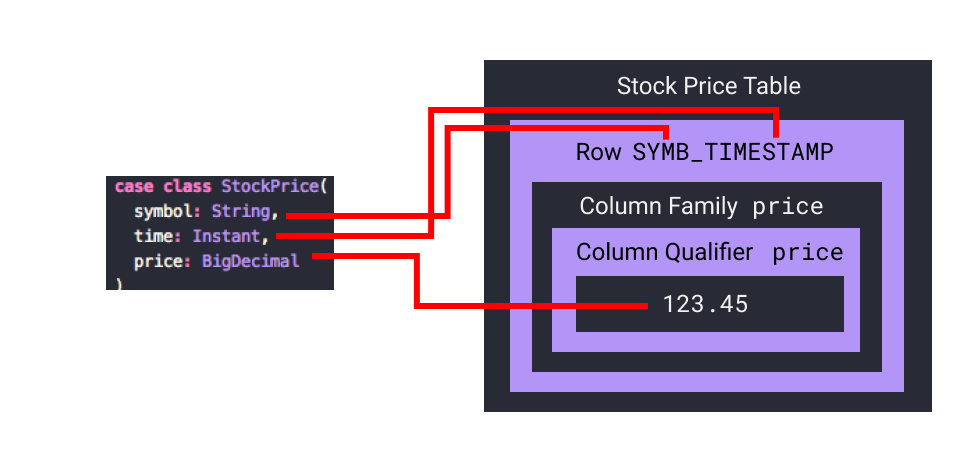
\includegraphics[max width=\textwidth]{stockPriceSchema}
  \end{center}
  \caption{The stock price data structure as a Scala case class (left) mapped onto its corresponding database schema (right).}
\end{figure}

\subsubsection{Opinion Aggregation}

The Opinion Aggregation component is responsible for storing and retrieving microblog posts from our database, performing sentiment analysis on those posts, and aggregating sentiments towards a particular stock symbol. A structure is defined to represent a microblog post, and a matching schema defines how it is stored in our database. Additionally, we represent the author of a microblog post as a structure of its own, even though it only contains one field at this point. Figure~\ref{microblogPostSchema} shows both the structures and schema and how to convert between the two. The conversion between the CSV of StockTwits data from 2014 provided by our client to the microblog post structure described above is done by parsing each row of the CSV and extracting the columns that correspond to the post id, text content, symbols mentioned, tagged sentiment, time, and author id. These columns translate directly into values stored in the \texttt{MicroblogPost} data structure.

Aggregating the opinions of microblog authors requires many data structures. In order to future-proof our implementation for the support of live data, we are modeling the opinion aggregation as an online algorithm so it processes input incrementally and doesn't need to have all posts available at the start of execution. This decision influences the intermediate values used in the calculation of the aggregate sentiment and the data structures required to represent them. The aggregate sentiment of a stock requires that we know the sum of the post author's weight multiplied by the order in which each post that mentions the stock with the same sentiment was posted. Since we only need the sum of these, we don't need to store every post in the time interval with its associated order. In order to know the order in which each post referencing a particular stock symbol and with a particular sentiment was created, we can store these values in a map with keys taking the form of a tuple containing the symbol and sentiment and values being an integer. Additionally, we need to store each author's weight. This can be represented by a map of microblog authors to an object that calculates the author's weight incrementally. An author's weight is calculated by dividing their average prediction score by the standard deviation of their prediction scores. The object that calculates the author's weight must store enough data to calculate the average and standard deviation of the set of prediction scores incrementally (i.e. adding one score at a time). The score of a prediction is only available after we know if the prediction was correct or not, which happens after a confirmation time window. Therefore, we also need to queue up posts until after the confirmation window in order to update each author's weight.

% Figure - microblogPostSchema (w/ Author)
\begin{figure}[h]
  \label{microblogPostSchema}
  \begin{center}
    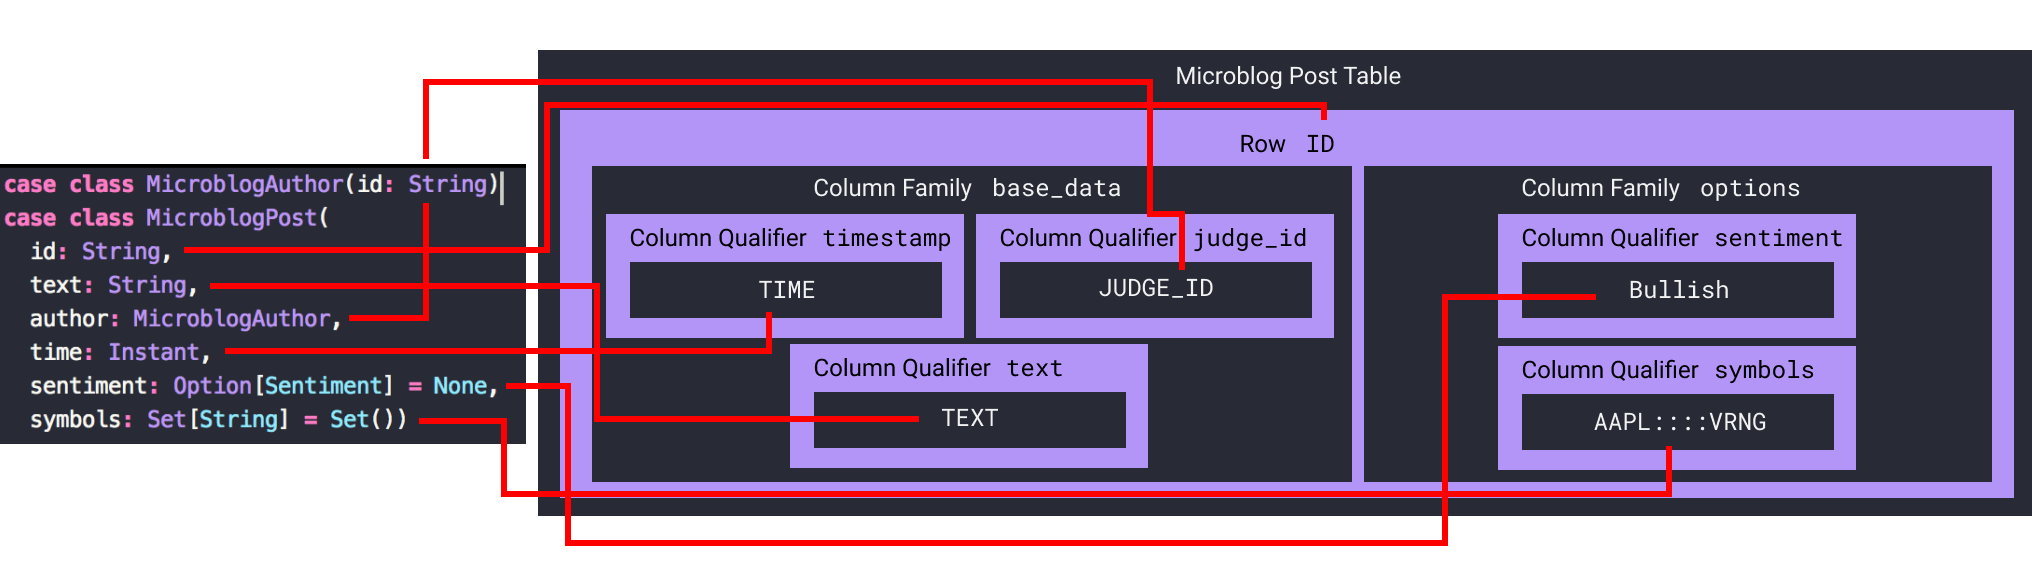
\includegraphics[max width=\textwidth]{microblogPostSchema}
  \end{center}
  \caption{The \texttt{MicroblogPost} and \texttt{MicroblogAuthor} data structures (left) mapped onto the corresponding database schema (right).}
\end{figure}

\subsubsection{Trading Simulation}

One of the main structures required in the Trading Simulation is the virtual portfolio. Storing a virtual portfolio involves storing the amount of each stock that is owned, as well as the amount of cash available. This structure is shown in figure~\ref{portfolioStruct}. Because we've decided to model a trading strategy as a listener to trading events, we must define what a trading event is. A trading event is any action or occurrence that is recognized by a trading strategy. The structure of a trading event will be defined to contain a time (so that all events are guaranteed to be sorted by their time of occurrence). Other than that, any implementation of a trading event may contain any arbitrary data. For example, a microblog event would be an implementation of a trading event that contains a microblog post. Trading event emitters create iterators of trading events (that are ordered by time). In order to process each event in order from all the emitters efficiently, a min priority queue that is sorted by the event time will be used to store the next event from each emitter. When an event is pulled from the priority queue, it will be processed by the strategy and then the next event from that emitter is inserted into the queue. This process repeats until there are no more events available.

% Figure - portfolioStruct
\begin{figure}[h]
  \label{portfolioStruct}
  \begin{center}
    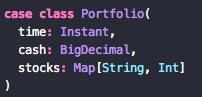
\includegraphics[max width=\textwidth]{portfolioStruct}
  \end{center}
  \caption{The virtual portfolio data structure.}
\end{figure}

\subsection{Data Flow}

This section gives a detailed view of how data flows between each component of the system.

\subsubsection{Pricing Data}

Data within the pricing data component flows into our system through external sources of prices. As described in previous sections, these sources consist of the Yahoo and Google Finance APIs. Data from these sources is processed and stored into HBase tables. Then, the stock price information flows out of the pricing data component through an interface than pulls the data from the appropriate HBase table.

\subsubsection{Opinion Aggregation}

External sources of microblog posts flow into the opinion aggregation component. As described in previous sections, the microblog data that we use is a set of posts from the StockTwits site in CSV format. These posts are processed and stored in an HBase table. An interface that pulls these posts from our database is provided so that other components can easily make use of this information. A utility is provided that analyzes the sentiment of a post. An additional utility calculates the aggregated sentiment towards a stock from a set of microblog posts. Both of these utilities receive microblog posts from another component (the Trading Simulation component) and return additional information (a sentiment or the current set of aggregated sentiments).

\subsubsection{Trading Simulation}

As discussed earlier, in the trading simulation component, trading events flow into a trading strategy object. In response to these events, a trading strategy will manipulate virtual portfolio objects to execute transactions. When executing transactions, the portfolio will use an interface provided by the pricing data component to get the current price of a particular stock. Additionally, trading strategies may use interfaces provided by the opinion aggregation and pricing data components as factors in their decision making.

\subsection{Group Roles}

Apart from Saurabh and Eric, we have a four person team to which we can delegate tasks. Joseph Watts functions as the Data Processing Specialist, which leads the effort on any interactions with the distributed data processing aspect of this project. This will require proficiency with Spark and HBase. Nick Anderson is our Portfolio Management and Machine Learning specialist. Nick will develop the portfolio management system that was detailed earlier and will assist Joseph Mehr in developing and researching machine learning algorithms. Joseph Mehr will specialize in machine learning and will specifically organize the effort behind implementing a Support Vector Machine (SVM). Connor Asbill is our Data Aggregation Researcher. His role involves researching new ways to best aggregate the data that we obtain (tweet sentiments, judge reliability scores, stock price changes, etc) to make informed trading decisions. On top of all of our roles, each of us is responsible for participating in the literature survey that is ongoing throughout this project.

\subsection{Timeline}

A timeline of milestones that plan out the course of our project can be seen below. Our group plans to meet once a week to delegate tasks and review work and research that has been done independently.

\begin{itemize}
\item Feb 15 - Draft Trading Simulation \& Pricing Data
  \begin{itemize}
    \item Before we can evaluate any trading strategy, we need to develop a system that simulates the trading environment (by replaying historical events and allowing a strategy to buy/sell stocks). By February 15th, we want to have an initial draft of the implementation of these pricing data and trading simulation components.
  \end{itemize}
\item Mar 1 - Complete Trading Simulation \& Pricing Data
  \begin{itemize}
  \item By March 1st, we want to have the pricing data and trading simulation components completed, so that we can start to implement and test trading strategies on top of this framework.
  \end{itemize}
\item Mar 15 - Complete Opinion Aggregation \& Baseline Strategy
  \begin{itemize}
  \item By March 15th, our goal is to complete our implementation of the opinion aggregation model laid out by \textit{CrowdIQ: A New Opinion Aggregation Model} \cite{crowdiq}.
  \item Additionally, we want to have the trading strategy described by this paper implemented by then.
  \end{itemize}
\item Apr 1 - Research and Start Implementing Trading Strategies
  \begin{itemize}
  \item From March 15th to April 1st, we'd like to have completed our research on trading strategies. By this time, our goal is to have identified three trading strategies and start on their implementation.
  \end{itemize}
\item Apr 15 - Complete Implementation and Analysis of Trading Strategies / Assemble Presentation
  \begin{itemize}
  \item By April 15th, our goal is to have working implementations of the trading strategies and analyze their results for the year of 2014.
  \item Additionally, we want to assemble the presentation that we will be giving to the rest of our capstone class on our work.
  \end{itemize}
\item Apr 25 - Complete Documentation of Work in Final Report
  \begin{itemize}
  \item By April 25th, we want to have completed our documentation for users and developers who are interested in our work.
  \end{itemize}
\end{itemize}


%%% Local Variables:
%%% mode: latex
%%% TeX-master: "../report"
%%% End:
